\documentclass{beamer}
%Information to be included in the title page:
\title{Analytic sets}
%\author{Anonymous}
%\institute{Overleaf}
\date{13.06.2025}

\usepackage{amsmath}
\usepackage{amsfonts}
\usepackage{amssymb}
\usepackage{amsthm}
\usepackage{euscript}
\numberwithin{equation}{section}
\usepackage{mathtools}
\usepackage{mathrsfs}
% Theorem-Umgebungen ------------------------------------
\usepackage{thmtools}




\begin{document}

\frame{\titlepage}

\begin{frame}
\frametitle{Mikhail Souslin and Nikolai Luzin}
\begin{figure}[h]
		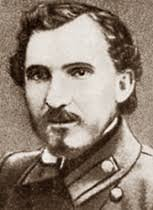
\includegraphics[width = 0.45\linewidth]{souslin}
		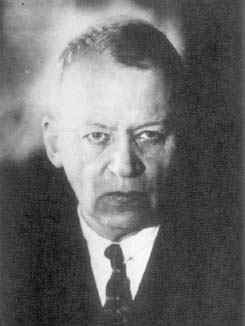
\includegraphics[width = 0.465\linewidth]{luzin}
\end{figure}
\end{frame}

\begin{frame}{Sur les fonctions représentables analytiquement}
	\begin{figure}
		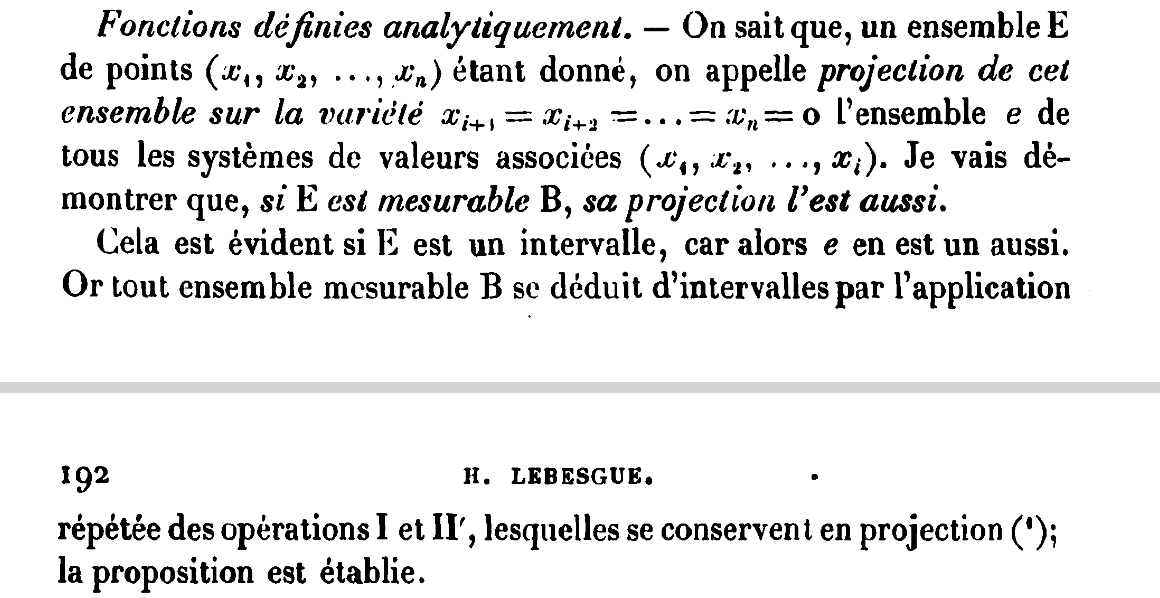
\includegraphics[width = 0.9\linewidth]{lebesgue_lemma}
	\end{figure}
	
\end{frame}

\begin{frame}{projections of Borel sets}
	lustige Grafik
\end{frame}


\begin{frame}{$\mathbb{N}^\mathbb{N}$ is a Polish space}
\begin{definition}[metric]
	A metric on $X$ is a function  $d: X \times X \to \mathbb{R}^+$, such that:
\begin{itemize}
	\item $d\left( x,y \right) = 0 \iff x = y$
	\item $d\left( x,y \right) = d\left( y,x \right) $
	\item $d\left( x,z \right) \leq d\left( x,y \right) + d\left( y,z \right) $ 
\end{itemize}
\end{definition}

\begin{definition}[complete]
	A metric space $\left( X,d \right) $ is complete, if every Cauchy sequence converges
\end{definition}

\begin{definition}[separable]
	A topological space $X$ is separable, if it contains a countable dense subset
\end{definition}

\end{frame}

\begin{frame}{Important results}
	\begin{theorem}
		Let $A$ be a nonempty Analytic subset of a Polish space $X$. Then there exists continuous function $f: \mathbb{N}^{\mathbb{N}} \to X$, such that $f\left( \mathbb{N}^{\mathbb{N}} \right) = A$
	\end{theorem}
\end{frame}


\begin{frame}{important results}
\begin{theorem}
	Each uncountable Polish space $X$ contains a homeomorphic copy of  $\mathbb{N}^\mathbb{N}$
\end{theorem}
\end{frame}


\begin{frame}{Universal set}
	\begin{theorem}
		There exists a set $M$, which is universal for the analytic sets in  $\mathbb{N}^\mathbb{N}$
	\end{theorem}
\end{frame}



\end{document}
